\documentclass[a4paper,10pt,oneside,titlepagethebibliography,]{article}
% Controle das margens
\usepackage{geometry}
\geometry{verbose,a4paper,tmargin=3cm,bmargin=2cm,lmargin=2cm,rmargin=2cm,headsep=5mm,footskip=0cm}
% Localização
\usepackage[brazil]{babel} % português do Brasil. 
\usepackage[T1]{fontenc} % fontes com acentos no PDF
\usepackage{ucs}
\usepackage[utf8x]{inputenc}
\usepackage{indentfirst}
\usepackage{moreverb}
% Controlar linhas orfas e viuvas
\clubpenalty=10000
\widowpenalty=10000
\displaywidowpenalty=10000
% Formatar notas de rodape
\usepackage[hang]{footmisc}
\setlength{\footnotemargin}{1em}
% Matemática
\usepackage{amsmath}
\usepackage{amsfonts}
\usepackage{amssymb}
% Imagens
\usepackage{graphicx}
% Extras
\newcommand{\HRule}{\rule{\linewidth}{0.5mm}}
\usepackage{listings}
\lstset{frame=single,numbers=left}
\renewcommand{\topfraction}{0.85}
\renewcommand{\textfraction}{0.1}
\renewcommand{\floatpagefraction}{0.75}
% Informações
\author{Gustavo Campos Ferreira Guimarães}
\title{Recuperação de Arquivos de Áudio Usando Splines Cúbicos}

\begin{document}
\begin{titlepage}
\begin{center}

\textsc{Universidade Federal de Minas Gerais}
\textsc{Departamento de Ciência da Computação}\\[1.5cm]
\textsc{\Large Análise Numérica: Trabalho Prático II}\\[3.0cm]


% Title
\HRule \\[1.5cm]
%{ \huge \bfseries Lager brewing techniques}\\[0.4cm]
{\huge Recuperação de Arquivos de Áudio \\ Usando Splines Cúbicos}\\[1.5cm]
\HRule \\[3.0cm]

% Author and supervisor
\begin{minipage}{0.4\textwidth}
\begin{flushleft} \large
\emph{Autor:}\\
Gustavo Campos Ferreira Guimarães
\end{flushleft}
\end{minipage}
\begin{minipage}{0.4\textwidth}
\begin{flushright} \large
\emph{Matrícula:} \\
2005041291
\end{flushright}
\end{minipage}\\[1.5cm]
Documentação feita em \LaTeX

\vfill

% Bottom of the page
{\large \today}

\end{center}

\end{titlepage}
\tableofcontents
\clearpage
\section{Introdução}
\subsection{Áudio Digital}
Desde o aparecimento dos primeiros computadores de tamanho e preço reduzidos, compatíveis com o 	poder aquisitivo da população mediana, em especial dos países desenvolvidos, suas utilidades para o entretenimento começaram a ser exploradas. Jogos, vídeos, música e várias outras aplicações neste que é um dos ramos mais lucrativos do planeta possuem suas versões digitais, aplicadas de uma forma ou de outra a algum tipo de computador pessoal, dos tão comuns PC's e consoles de video-game até os novatos Media Centers e Home Theaters.

O áudio digital foi um dos pioneiros nessa nova onda de entretenimento digital. Primeiramente com os primeiros e rudimentares sons sendo gerados por 'tiques' em auto-falantes simplórios. Os primeirs sons de computador comumente eram loops do tipo \textit{for} ou \textit{while}, gerando em intervalos de tempo certos valores numéricos, que eram convertidos em sinais elétricos e enviados aos auto-falantes. Um método bastante trabalhoso para qualquer um que se aventurasse no áudio digital.

Com o tempo, sobretudo após os computadores se tornarem mais robustos, as técnicas de amostragem de áudio surgiram e possibilitaram o boom do áudio digital, que culminou na década de 90 com o aparecimento do Compact Disc, que revolucionou a forma das pessoas ouvirem música em casa. Seguido pouco depois pelo MP3, que na verdade teve o efeito contrário, o CD foi o responsável por uma melhoria significativa na qualidade do áudio acessível ás pessoas, acostumadas ao discos de vinil, que, apesar de usarem áudio analógico, sofriam muito facilmente os efeitos das intempéries de mau uso e do tempo, já que exigiam o atrito entre as superfícies do disco e da agulha.

\subsection{O Problema}

Apesar da aparente melhoria na qualidade de som, o áudio digital mascara uma muitas vezes considerável perda nessa qualidade. Arquivos de áudio digital na verdade são amostragens dos sons reais, pontos discretos de uma onda sonora contínua.

Basicamente, o processo de amostragem de som consiste em capturar as ondas sonoras com um dispositivo de entrada, usualmente um microfone, e em certos intervalos de tempo gravar o valor numérico da amplitude da onda, numa determinada escala. No fim, tem-se uma amostragem de pontos que se aproximam da onda original. Quanto mais pontos, ou seja, quanto maior a taxa de amostragem, melhor a qualidade do som, em teoria.

Em geral uma taxa de 44100Hz (44100 pontos por segundo) é a utilizada na indústria fonográfica para realizar a amostragem de som digital. Essa é a qualidade padrão dos CD's de áudio e dos arquivos de MP3 (a perda de qualidade destes se deve a outros fatores, que fogem do escopo desta análise). Isso gera um som bastante fiel, indiferenciável para a maioria dos ouvidos humanos (há sempre quem diga que pode diferenciar o som original do digital).

Apesar de o áudio digital gerado não ser 100\% fiel à onda sonora original, a qualidade obtida nos CD's é bem superior, em geral, á obtida em discos de vinil (existem discos especiais, mais resistentes a risco, e uma nova tecnologia de leitura de discos de vinil que não necessita do contato entre o dispositivo de leitura e o disco), já que a leitura é feita através de um laser, que não toca a superfície do disco, como fazia-se com as antigas vitrolas, evitando assim ruídos devido ao atrito.

O problema real nasce quando por algum motivo, a taxa de amostragem do arquivo de áudio é inferior à um certo valor (aproximadamente 90\% dos 44100Hz). A partir daí a degradação do áudio começa a ser notável pelas pessoas comuns, o que gera insatisfação de várias formas. Há ainda aqueles sedentos pelo áudio perfeito, chamados de audiófilos, que estão sempre em busca de áudio de maior pureza e fidelidade. Para esses casos foi desenvolvida a técnica da interpolação de áudio.

A maioria dos CD-players de qualidade hoje possui em seu hardware um chip que faz a interpolação do áudio de CD's e arquivos de áudio digital em geral. Não tive acesso às técnicas utilizadas por esses aparelhos, por isso resolvi implementar minha própria técnica, como forma de experimentar o poder da interpolação por \textit{Splines Cúbicos}, e avaliar o resultado criticamente.

\section{Abordagem de Solução}

A idéia básica por trás da interpolação de áudio é bastante simples: utilizar técnicas de interpolação de curvas para, de posse dos pontos amostrados da onda original, tentar aproximar outros pontos não presentes na amostragem, de forma a compor uma nova onda, mais próxima da onda original, tentando assim melhorar a fidelidade do som. 

É possível usar várias técnicas de interpolação para isso, que não é uma tarefa fácil. Ondas sonoras possuem uma quantidade elevadíssima de picos e vales, o que diminui consideravelmente a eficiência de qualquer algoritmo de interpolação, afinal normalmente esses algoritmos em geral usam um processo de \emph{ligar os pontos} para poder conectar os pontos de amostragem e formar uma curva.

Escolhi o método de splines cúbicos pois sua característica principal é criar curvas mais suaves, partindo de um número maior de pontos de amostragem. A minha intenção com isso era conseguir tentar recuperar os picos da onda sonora. Para isso escolhi a implementação de splines extrapolados, pois sua característica de extrapolação poderia ser útil para obter esses picos e vales.

\subsection{Splines Cúbicos}

Os \textit{splines cúbicos} são uma técnica de interpolação que consiste em utilizar uma série de polinômios interpoladores cúbicos para aproximar os pontos interpolados, a característica principal desta técnica é gerar curvas bastante suaves, com um relativamente baixo custo computacional. os \textit{splines} são o algoritmo padrão de interpolação de diversos softwares matemáticos, a citar o \emph{MatLab} e o usado neste trabalho: \emph{GNUplot}.

As características dos \textit{splines} advêm das suas condições de existência, basicamente duas:

\begin{itemize}{}{}
\item Dois \textit{splines} consecutivos devem, obrigatoriamente, passar pelo mesmo ponto
\item As derivadas de dois \textit{splines} consecutivos devem ser iguais
\end{itemize}

Dessa forma garante-se a continuidade dos \textit{splines} bem como a máxima aproximação de suas inclinações e curvaturas. Existem vários tipos de \textit{splines}, dentre os quais foram estudados os naturais e extrapolados. Para esta implementação, optei pelos \textit{splines extrapolados} na esperança de que a geração de valores ligeiramente excessivos nas bordas me ajudasse a conseguir melhores aproximações para os picos e vales das ondas sonoras. Certamente o ideal seria comparar vários métodos de interpolação, não apenas \textit{splines}, nem tão somente apenas \textit{splines extrapolados}, mas as limitações de tempo inerentes à condição de estudante impediram tal extrapolação.

\section{Modelagem Matemática}

Sendo um método que não envolve matemática avançada, a interpolação não requer uma modelagem matemática muito complexa. Descreverei brevemente, quase que em citação do livro didático adotado em sala de aula, a técnica usada especificamente pelos \textit{splines extrapolados} para obter suas aproximações. Excluindo-se as provas envolvidas, vamos às fórmulas:

Um \textit{spline cúbico} é essencialmente um polinômio da forma:
\begin{center}
\fbox{$ s_i = a_i (x-x_i)^3 +  b_i (x-x_i)^2 + c_i (x-x_i)+d_i, i = 0,1,2,...,n-1$}
\end{center}

Lembrando que os valores dos \textit{splines} nos extremos de cada intervalo devem ser iguais, bem como suas derivadas primeira e segunda nesses mesmos pontos. Partindo desse pressuposto obtemos as fórmulas para os coeficientes \textit{a,b,c} e \textit{d} de cada \textit{spline}:

\begin{center}
\fbox{$ a_i =  \frac{s_{i+1}^n(x_{i+1}) -s^n_i(x_i)}{6h_i},i = 0,1,2,...,n-1$}
\end{center}

\begin{center}
\fbox{$ b_i = \frac{s_i^n(x_i)}{2}, i = 0,1,2,...,n-1$}
\end{center}

\begin{center}
\fbox{$ c_i = \Delta y_i - \frac{s_{i+1}^n(x_{i+1})+2s^n_i(x_i) }{6}h_i ,i = 0,1,2,...,n-1$}
\end{center}

\begin{center}
\fbox{$ d_i = y_i, i = 0,1,2,...,n-1$}
\end{center}

onde \fbox{ $ h_i  = (x_{i+1}) - x_i $ }, e \fbox{$\Delta y_i = \frac{y_{i+1}-y_i}{h_i}$}

Que nos dá um sistema linear subdeterminado com quatro incógnitas para cada spline, o que é um problema, visto que com isso falta-nos duas equações para poder determinar completamente o sistema.

A estratégia utilizada no \textit{spline cúbico extrapolado} é igualar as derivadas terceiras dos extremos dos \textit{splines}, eliminando assim duas variáveis e possibilitando sua solução. Como o sistema linear resultante é relativamente simples, só possuindo a diagonal principal e as sub-diagonais imediatamente inferior e superior a ela, o esforço computacional necessário para sua solução é relativamente pequeno, se comparado à solução de sistemas lineares convencionais equivalentes, tornando viável a solução de 

\section{Implementação}

A implementação so método supracitado foi feita utilizando Fortran90, por ser mais flexível e eficiente que o Fortran77. Além disso, os compiladores de Fortran atuais possuem um suporte parcial ao Fortran77, podendo acarretar em problemas. O código foi compilado tanto usando o compilador livre \emph{gfortran}, parte do pacote de compiladores livres \emph{gcc}, quanto na plataforma fechada \emph{Intel Fortran Compiler}, distribuida gratuitamente para uso não comercial.

Não posso avaliar com precisão o desempenho de ambos os compiladores. O compilador da Intel gerou um código ligeiramente mais eficiente na maiora dos casos, mas o \emph{gfortran} foi superior em algumas ocasiões, sobretudo na maior massa de dados que eu dispunha, com cerca de 800Kb.

A seguir seguem-se os detalhes da implementação.

\subsection{Decisões de Implementação}

Devido a alguns problemas encontrados, algumas decisões precisaram ser tomadas para possibilitar a implementação do programa. Abaixo defino as decisões que considero mais relevantes:

\subsubsection{Scripts Auxiliares}

Para conseguir manipular as massas de dados, foi necessária a criação de diversos scripts, de forma a automatizar o processo de geração, compilação e plotagem dos dados. São scripts relativamente simples, usando linguagem bash e os softwares gnuplot e sox, comentados à frente.  O principal deles é o script \textit{geradados.sh} que consiste no código a seguir.

Uma das funções do script é "degradar" um amostra de áudio de 44100hz, gerando versões com menor amostragem, de forma que eu possa aplicar a interpolação nas amostras degradadas e avaliar sua aproximação à amostra original.

\clearpage
\lstset{language=bash}
\lstinputlisting{../../scripts/gera-dados.sh}
\subsubsection{Alocação Estática}

A princípio, como pode ser visto no código comentado, utilizei a estrutura \texttt{ALLOCATABLE} do Fortran, que permite alocar dinamicamente memória. Isso me possibilitava ler primeiramente do arquivo a quantidade de linhas a serem lidas, e em seguida alocar a quantidade de memória exata para a leitura, usando o comando \texttt{ALLOCATE}. Infelizmente a quantidade de problemas ocorridos, em especial devido a acessos indevidos à memória, me fez optar pela forma clássica de alocação estática de arrays, estipulei então um valor teto de 40000 espaços, suficiente para analisar alguns segundos de áudio.

\subsubsection{Argumentos em Linha de Comando}

Como faria testes com arquivos diferentes várias vezes, e pretendia automatizar o processo através de scripts, decidi passar os arquivos de entrada e saída como parâmetros de linha e comando. Isso é facilmente obtido através do uso da função \texttt{GETARG}, em conjunto com a função \texttt{IARGC}.

\subsubsection{Seno}

Para melhor ilustrar o funcionamento do programa, decidi rodá-lo sobre uma função simples para que os resultados fossem melhor visualizados. Escolhi a função $ \sin{30x}$ , pois possui uma periodicidade razoável e é regular o suficiente para deixar os gráficos plotados claros e visíveis. Para gerar os pontos, implementei um pequeno programa em fortran:

\lstinputlisting{../../seno.f90}

\subsection{Softwares Auxiliares}

Dois softwares de terceiros foram necessários para a implementação do projeto (estou excluindo obviamente editores de texto, compiladores e editores latex). Estes e suas funções são descritos abaixo:

\subsubsection{SoX}

O Sox é um projeto de software livre para conversão de arquivos de áudio digital. Fiquei muito satisfeito ao descobrir que ele é poderoso o suficiente para, a partir de um arquivo de áudio, gerar um arquivo de dados consistindo da amplitude da onda pelo tempo, extamente o que eu precisava para extrair dados numéricos de arquivos de áudio. Como também pode fazer o caminho contrário, o Sox me possibilitou verificar na prática, de forma auditiva, a eficiência do meu método.

\subsubsection{GNUPlot}

O GNUplot é um software livre renomado para plotagem de dados matemáticos tanto em 2d quanto em 3d. Ele é capaz de gerar diversos tipos de imagens e arquivos, a partir de dados experimentais, massas de dados numéricos e funções predefinidas. É ainda capaz de utilizar vários métodos numéricos, entre eles a própria interpolação por \textit{splines cúbicos}. Todos os gráficos usados foram feitos com ajuda do GNUplot.

\subsection{Formatos de Dados}

Formatos de dados bastante simples foram usados. Como amostragem, escolhi alguns arquivos WAV, que tratam-se de áudio digital sem compressão, para fazer os testes. A princípio havia tentado com pequenos trechos de músicas, mas tendo em vista que a quantidade de dados contida era imensa, preferi optar por \textit{samples} de instrumentos, como notas únicas de bateria e teclado. Como o resultado é bastante similar para todas, estou incluindo apenas dois exemplos nesta documentação.


\subsubsection{Entrada e Saída de Dados}

Tanto a entrada como a saída do programa consistem, basicamente, de arquivos de texto em duas colunas, sendo a primeira uma lista de abcissas, e a segunda uma lista de ordenadas correspondentes. Nestes arquivos, as abcissas equivalem ao tempo, enquanto as ordenadas à amplitude da onda. Este formato é comum tanto ao GNUplot quanto ao meu programa, e são gerados automaticamente pelo Sox a partir de arquivos de áudio.

No caso da entrada do meu programa, precisava de uma primeira linha que me dissesse quantos pontos devo ler. inclui e exclui essa linha conforme necessidade usando o comando \texttt{sed} do Linux, como pode ser observado em meus scripts.

\subsection{Sintaxe de Execução}

A sintaxe de execução do programa é bastante simples e consiste da forma:

\begin{center}
\fbox{\texttt{cubicsplines arquivo-de-entrada arquivo-de-saida}}
\end{center}

Sendo os argumentos auto descritivos.

\section{Resultados}

Abaixo uma descrição e comentários dos resultados obtidos.

\subsection{Testes Realizados}

Escolhi arbitrariamente dois arquivos de áudio, baseado na diferença audível entre a amostra degradada. Primeiramente temos uma comparação dos resultados aplicados a uma função simples: $\sin{30x}$, em seguida aplicadas aos arquivos de áudio. Vale lembrar que foi preciso aumentar consideravelmente o zoom nos casos dos arquivos de áudio para possibilitar alguma diferenciação visual.

Extrai as legendas incluidas automaticamente pelo GNUplot, pois confundiam a visualização, devido à impressão monocromática.

\clearpage
\subsection{Resultados Obtidos}

\begin{figure}[h]
\begin{center}
\leavevmode
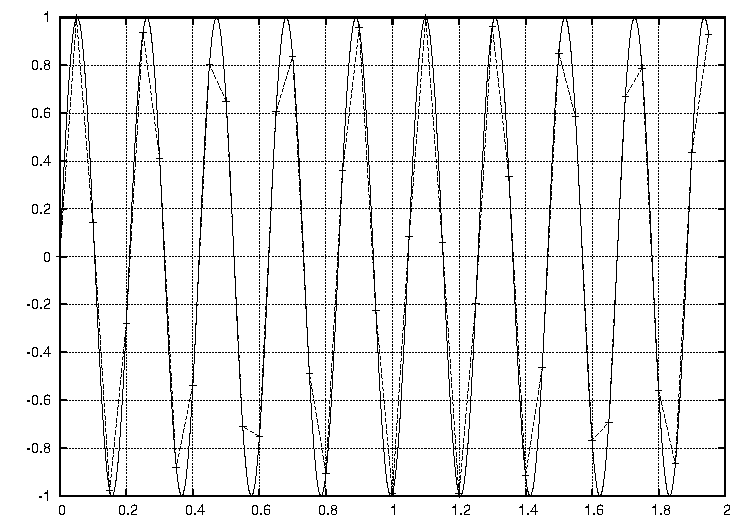
\includegraphics[scale=1]{../img/seno-normal.pdf} 
\caption{Neste gráfico, a linha pontilhada é a amostra degradada do seno, comparada à função seno original}
\end{center}
\end{figure}


\begin{figure}[h]
\begin{center}
\leavevmode
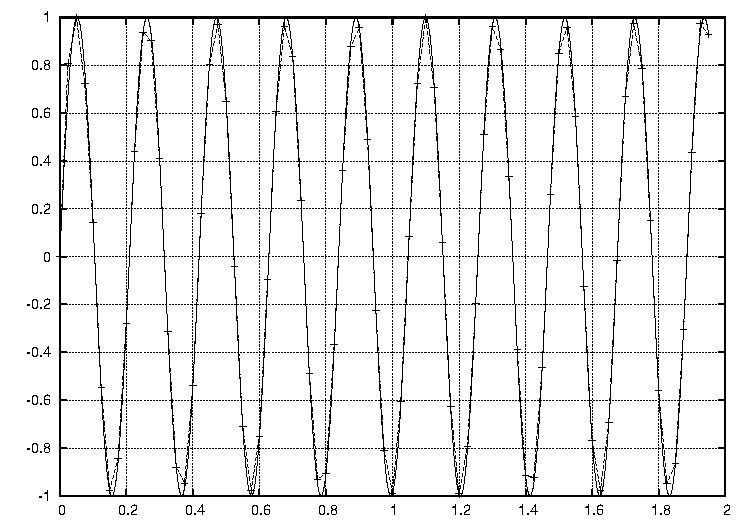
\includegraphics[scale=1]{../img/seno-interp.pdf} 
\caption{Neste gráfico, a linha pontilhada é a amostra interpolada do seno, comparada à função seno original}
\end{center}
\end{figure}

\clearpage

\begin{figure}[h]
\begin{center}
\leavevmode
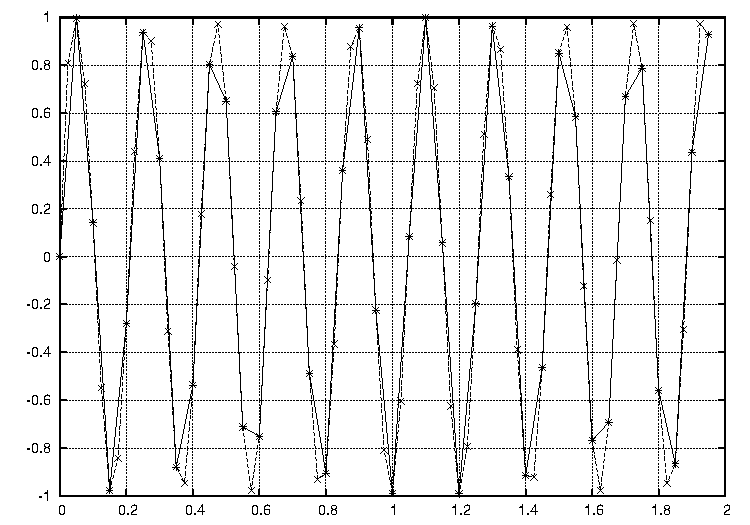
\includegraphics[scale=1]{../img/seno-comp.pdf} 
\caption{Neste gráfico, a linha pontilhada é a amostra interpolada do seno, comparada à amostra degradada}
\end{center}
\end{figure}

\begin{figure}[h]
\begin{center}
\leavevmode
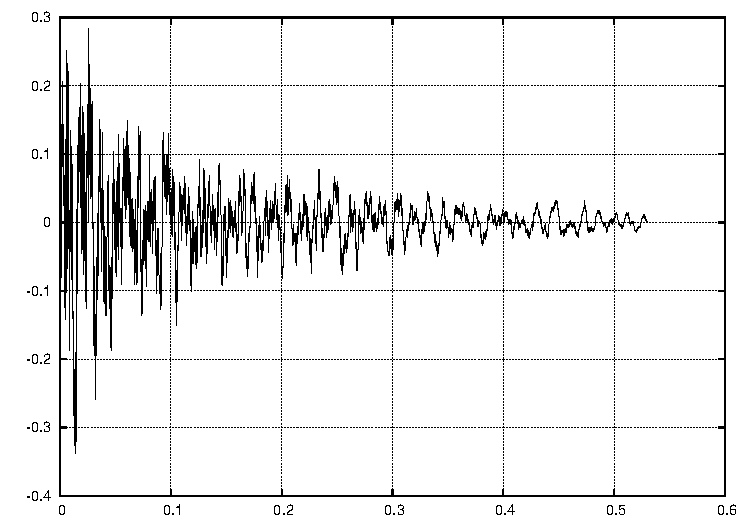
\includegraphics[scale=1]{../img/drum01-22050-normal.pdf} 
\caption{Amostra degradada de uma bateria a 22050Hz, é difícil notar alguma coisa, pois é muita informação}
\end{center}
\end{figure}

\clearpage

\begin{figure}[h]
\begin{center}
\leavevmode
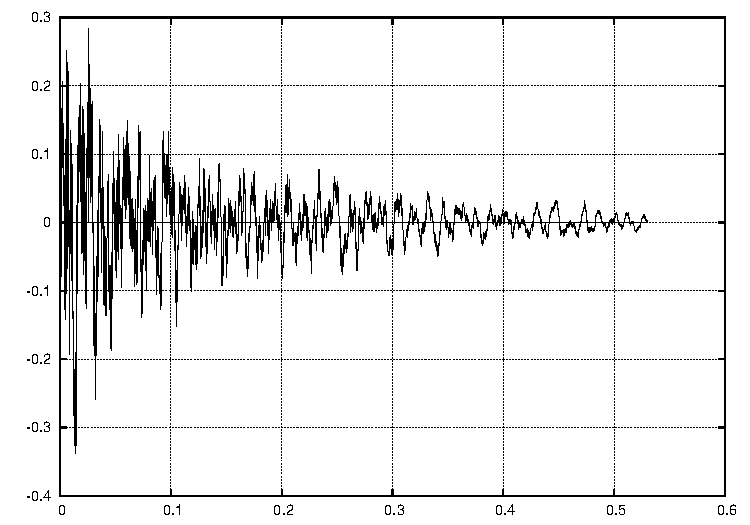
\includegraphics[scale=1]{../img/drum01-22050-interp.pdf} 
\caption{Amostra interpolada a partir do arquivo acima, aparentemente são iguais}
\end{center}
\end{figure}

\begin{figure}[h]
\begin{center}
\leavevmode
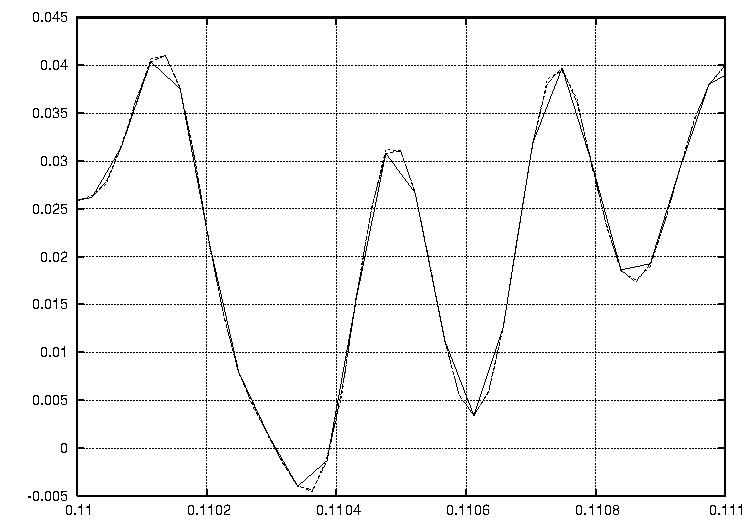
\includegraphics[scale=1]{../img/drum01-22050-comp.pdf} 
\caption{Fazendo um zoom vemos a diferença.  A linha tracejada (interpolada) e a pontilhada (original) estão quase coincidentes, e relativamente espaçadas da amostra degradada (linha contínua)}
\end{center}
\end{figure}

\clearpage

\begin{figure}[h]
\begin{center}
\leavevmode
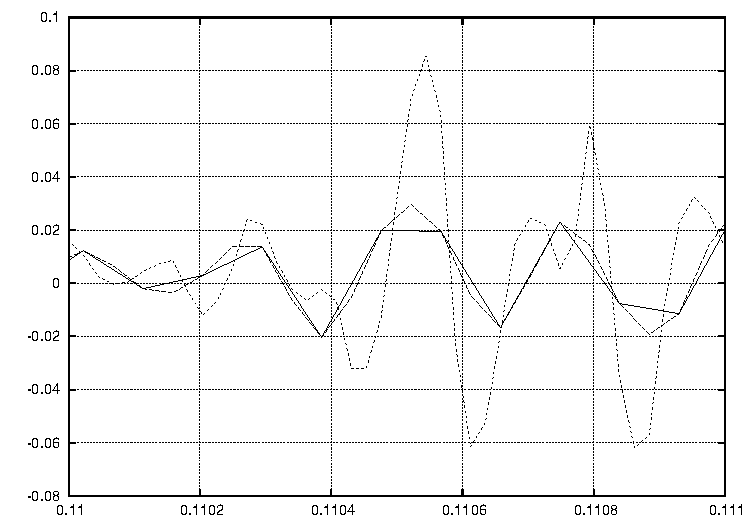
\includegraphics[scale=1]{../img/drum03-11025-comp.pdf} 
\caption{Amostra de um outro áudio, dessa vez mais degradada - a 11025Hz - nessa amostra tantos dados foram perdidos, que a melhoria da linha interpolada (tracejada) deixa muito a desejar à original (pontilhada) mesmo estando razoavelmente melhor que a versão degradada (linha contínua)}
\end{center}
\end{figure}

\subsection {Comentários}

Podemos notar claramente em todos os exemplos que a amostra interpolada possui uma fidelidade maior com a amostra real. Isso é claramente visível na função seno, mas podemos inferir também a mesma conclusão para as amostras sonoras, uma vez que, mesmo não estando de posse da onda original, a amostra reconstituida se aproximou da amostra não degradada.

\section{Conclusão}

Analisando visualmente os dados, podemos concluir que a interpolação por \textit{splines cúbicos} dos arquivos de áudio foi um sucesso, e foi capaz de reconstituir uma parte considerável das ondas originais. Talvez se mais interpolações fossem feitas, uma sobre a outra, os resultados fossem melhores, mas infelizmente não houve tempo hábil para fazê-lo.

Infelizmente porém, fui incapaz de perceber qualquer diferença notável no som gerado pelas amostras degradadas e pelas amostras reconstituidas. Muito provavelmente este fato está conectado à incapacidade de se gerar os picos e vales mais extremos que foram perdidos na degradação da amostra de áudio. Tendo em vista que essa degradação chegou a 75\% em alguns dos meus testes, era de se esperar que fosse difícil reconstituí-los.

O resultado final porém foi bastante satisfatório, sobretudo como forma de testar, avaliar e compreender melhor o método de interpolação por \textit{splines cúbicos}, bem como de visualizar os resultados de sua aplicação numa situação real.

\section{Código Fonte}

Estão anexos os códigos fontes implementados em Fortran90
\clearpage
\begin{thebibliography}{9}

	\bibitem{alhpaii}
		\emph{\LaTeX: Alpha II - Programming Information: Audio Interpolation}\\
		\texttt{http://www.alpha-ii.com/Info/AudioInt.html}
	\bibitem{gnuplotinfo}
		\emph{Gnuplot Homepage}\\
		\texttt{http://www.gnuplot.info}
	\bibitem{sox}
		\emph{Sox Project}\\
		\texttt{http://sox.sourceforge.net/}
	\bibitem{gnuplottut}
		\emph{Gnuplot: Not so frequently asked questions}\\
		\texttt{http://t16web.lanl.gov/Kawano/gnuplot/index-e.html}
	\bibitem{ffcampos2}
		Frederico Ferreira Campos filho;
		\emph{Algoritmos Numéricos}.
		LTC,
		Segunda Edição,
		2006.
\end{thebibliography}

\end{document}